\section{Common Geometries}

\subsection{Geometry From File}
To switch on the geometry definition from an external file, the messenger 
command 
\begin{lstlisting}
/MG/geometry/detector GeometryFile
\end{lstlisting}
has to be given. The name of the file containing the geometry to be read 
is set using the command 
\begin{lstlisting}
/MG/geometry/geometryFileName mygeometry.def
\end{lstlisting}
If the command \texttt{/MG/geometry/geometryFileName} is issued more than 
once, the file name is overwritten, and the last one is taken into account. 
If the general geometry has not been set with the command 
\texttt{/MG/geometry/detector GeometryFile}, the file name is anyway accepted 
but it is not used. If the file name is not given explicitly, the default 
\texttt{geometry.def} is looked for in the current directory. \\
It is possible to define an arbitrary 
number of boxes, cylinders and spheres. Volumes can be daughters of the 
world or of an other volume. In the latter case, it is possible to define 
``holes'' in a given volume. \\
An example of geometry definition file is the following: \\
\begin{lstlisting}
1 Crystal 2 1 0 SodiumIodide   
0. 0. 2.55 
2.55 5.10 0. 
0. 0. 0. 
2 Hole    2 0 1 Air             
0. 0. 0.65 
1.43 3.80 0.
0. 0. 0. 
\end{lstlisting}
Each volume is defined in four lines. \\
(1) The entries for the first line are:
\begin{itemize}
\item ordering number (int).
\item volume name (string). This is the name of the physical volume defined 
in the geometry. It can be used, for instance, for the uniform sampling 
routine. The names of the volumes should be different, though there is no 
specific control in the program. 
\item shape of the volume (int). The code is 1 for boxes, 2 for cylinders and 
3 for spheres. If the code is different from the values listed above, the volume  
is ignored.
\item sensitive detector flag (int). If the flag is 1, the volume is 
registered as a sensitive detector for the subsequent analysis. 
\item mother flag (int). If the flag is set to 0, the volume is placed inside the 
world volume. If the flag is a non-zero integer $n$, the volume is considered 
to be a daughter of the volume $n$. The mother volume must be defined 
\emph{before} the daughter one (namely, the ordering number of the Daugherty 
must be larger than $n$). It is possible to nest daughter volumes one inside 
the other.
\item material name. The material has to be included in the \mage database 
or defined using an external file, as described in Sect.~\ref{subsection:materials}.
\end{itemize}
(2) The second line contains the three coordinates of the volume center, given in cm (double). 
Coordinates are always expressed with respect to the mother volume reference system. \\
(3) The third line contains the three physical dimensions of the volume (double), given in cm. 
For boxes, the numbers are the sizes along the $x$, $y$ and $z$ axes, respectively. 
For cylinders, the first parameter is the radius, and the second the height (the 
third parameter is unused).  
For spheres, the first parameter is the radius, the other two are unused. \\
(4) The fourth line contains the three Euler angles (degrees) defining the volume rotation. 
The angles are always referred to the mother volume reference system. \\
The volumes defined in the external file are placed in a world volume made of air. The 
world volume is a cube of 5~m size. Therefore, the dimensions of the volumes in 
the file cannot exceed 5~m.\\
The geometry file presented above represents: a cylindrical sodium iodide detector (radius 
2.55~cm, height 5.10~cm) with a cylindrical hole (radius 1.43~cm, height 3.8~cm) displaced 
of 0.65~cm along the $z$-coordinate of the detector. The coordinates of the center of the 
detector are (0,0,2.55~cm) with respect to the world reference frame. The sketch of the 
geometry is displayed in Fig.~\ref{testgeometry}. \\
%%
\nopagebreak
\begin{figure}[tb]
\begin{center}
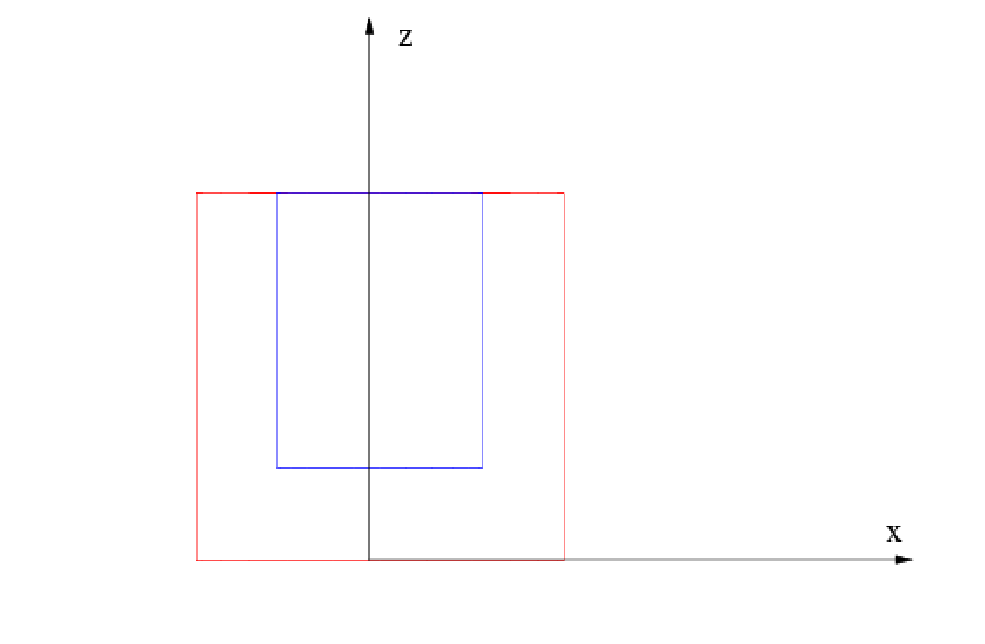
\includegraphics[height=10cm]{figures/geom-from-file}
\caption{Sketch of the setup geometry defined in \textsc{MaGe} with the external 
data files used as example in the text.}\label{testgeometry}
\end{center}
\end{figure}
%
\section{GERDA Geometries}
 
\subsection{GERDA Phase I}
\begin{lstlisting}
/MG/geometry/detector GerdaArray
/MG/geometry/detector/geometryfile geometry.dat
/MG/geometry/detector/matrixfile matrix_phase_i.dat
\end{lstlisting}
The standard GERDA setup (to be specified) including the detector
array (with cables and holders), the cooling liquid (argon), the
cryogenic tank, the water tank, the lock and the cleanroom. Also
included are the PMTs and the plastic scintillator on top of the
cleanroom. Parts of the infrastructure, in particular beams between
the cleanroom and the water tank, are also simulated. The detectors
are described in geometry.dat, the array configuration is described in
matrix\_phase\_xxx.dat\\

The Phase~I setup includes an array of 9 non-true coaxial
detectors. They are stacked in three strings of three detectors each.

\subsection{GERDA Phase II}
\begin{lstlisting}
/MG/geometry/detector GerdaArray
/MG/geometry/detector/geometryfile geometry.dat
/MG/geometry/detector/matrixfile matrix_phase_ii.dat
\end{lstlisting}

See GERDA Phase~I for the general setup. The Phase~II setup includes
five true coaxial and three non-true coaxial detectors per layer for
three layers in total. 

\subsection{GERDA Phase II Ideal}
\begin{lstlisting}
/MG/geometry/detector GerdaArray
/MG/geometry/detector/geometryfile geometry.dat
/MG/geometry/detector/matrixfile matrix_phase_ii_ideal.dat
\end{lstlisting}

See GERDA Phase~I for the general setup. The Phase~II ideal setup
includes seven true coaxial detectors per layer for three layers in
total.

\subsection{Test Stand Simple}
\begin{lstlisting}
/MG/geometry/detector MunichTestStand
/MG/geometry/teststand/teststandtype simple
\end{lstlisting}

Describes a ReGe detector with a source placed infront of it. The
source is surrounded by lead bricks. The distance between the crystal
and the source as well the distance between the source and the lead
bricks can be set by macro with
\verb*|/MG/geometry/teststand/crystaltosource| and
\verb*|/MG/geometry/teststand/sourcetobrick|, respectively. 

%\subsubsection{Test Stand Siegfried}
%FixME Jing
%\begin{lstlisting}
%/MG/geometry/detector MunichTestStand
%/MG/geometry/teststand/teststandtype siegfried
%\end{lstlisting}

\subsection{Test Stand LN2}
\begin{lstlisting}
/MG/geometry/detector MunichTestStand
/MG/geometry/teststand/teststandtype ln2
\end{lstlisting}

Simulates an unsegmented DSG p-type detector in the GERDAlinchen test
stand, i.e. a cryostat filled with liquid nitrogen. It includes an AEA
source inside the cryogenic liquid. 

\subsection{Heidelberg Detectors}
\begin{lstlisting}
/MG/geometry/detector Bruno
/MG/geometry/detector Corrado
/MG/geometry/detector Dario
\end{lstlisting}

Simulates the three main detectors used at Heidelberg for material screening.
Includes full models of shielding and samples. The samples can be defined
by the following command:
\begin{lstlisting}
/MG/geometry/dario/sample [sphere] [box] [tube] [sbox] [liquid] [twobox]
[marinelli] [custom]
\end{lstlisting}
For different detectors replace the detector name in the command (and all following commands) accordingly, e.g. for Bruno : \texttt{/MG/geometry/bruno/sample}.\\
Description of sample options :\\
(1) The default geometry option is \texttt{sphere}, which creates a sphere of fixed radius 0.1 $\mu$m. This is used only to put the volume \texttt{sample} out of way when generating gammas from a single point.\\
(2) The outer dimensions of geometry \texttt{box} can be set by the following self-explanatory commands:
\begin{lstlisting}
/MG/geometry/dario/boxwidth dimension [unit]
/MG/geometry/dario/boxheight dimension [unit]
/MG/geometry/dario/boxthickness dimension [unit]
\end{lstlisting}
(3) The geometry \texttt{tube} produces a cylinder with a possible concentric hole. The dimensions can be specified by the following parameters:
\begin{lstlisting}
/MG/geometry/dario/tubelength dimension [unit]
/MG/geometry/dario/tubeouterradius dimension [unit]
/MG/geometry/dario/tubeinnerradius dimension [unit]
\end{lstlisting}
(4) The geometry \texttt{sbox} is identical to \texttt{tube} (the same dimension-parameters apply), but adds a standard cylindrical
box used for measurements at MPIK laboratory (lid facing the detector). The position of the container changes according to the position of the sample, but the size is fixed, so it's users responsibility to ensure the \texttt{sample} volume fits inside and doesn't overlap with the container volume. The default dimensions of the sample cylinder correspond to the inner dimensions of the standard cylindrical box, so for samples which fill the inner volume completely, these parameters don't need to be specified.\\
(5) The geometry \texttt{liquid} is an extension of the \texttt{sbox} geometry. It subtracts a flat volume from the top of the sample, to simulate liquid not filling completely the volume of the standard box. For defining the liquid level, the command \texttt{/MG/geometry/dario/boxheight} is used. The value corresponds to liquid level measured from top (vertical dimension of the missing part).\\
(6) The geometry \texttt{twobox} adds two (empty) standard cylindrical containers in front of the detector.\\
(7) The geometry \texttt{marinelli} (not available for \texttt{Bruno} detector) is an extension of the \texttt{sbox} geometry. It creates a marinelli shaped sample (a box with a hole), with external dimensions defined by \texttt{boxwidth}, \texttt{boxheight} and \texttt{boxthickness} parameters, and internal hole depth and radius defined by \texttt{tubelength} and \texttt{tubeouterradius} parameters. The parameter \texttt{tubeinnerradius} is used to displace the hole from the center in vertical direction.\\
(8) The option \texttt{custom} selects additional geometry, which can't be described by previous commands, but has to be coded in the detector construction source file.\\
The following parameters define the sample position with respect to the center of the front 
detector window :
\begin{lstlisting}
/MG/geometry/dario/samplexpos dimension [unit]
/MG/geometry/dario/sampleypos dimension [unit]
/MG/geometry/dario/samplezpos dimension [unit]
\end{lstlisting}
The command:
\begin{lstlisting}
/MG/geometry/dario/samplematerial [material name]
\end{lstlisting}
defines the material of the sample. A material with the same name has to be defined in \texttt{MGGerdaLocalMaterialTable.cc} or from external file with the \texttt{/MG/geometry/addMaterial} command, as described in Sect.~\ref{subsection:materials}.\\
Additional commands can be used with detector \texttt{Dario} to adjust the parameters of the crystal:
\begin{lstlisting}
/MG/geometry/dario/detzpos dimension [unit]
\end{lstlisting}
Guidance: Sets the distance in \texttt{z} direction between the detector window and crystal surface.
\begin{lstlisting}
/MG/geometry/dario/deadthickness dimension [unit]
\end{lstlisting}
Guidance: Sets the dead layer thickness.
\begin{lstlisting}
/MG/geometry/dario/detdiameter dimension [unit]
\end{lstlisting}
Guidance: Sets outer diameter of the crystal (including dead layer).
\begin{lstlisting}
/MG/geometry/dario/detlenght dimension [unit]
\end{lstlisting}
Guidance: Sets lenght of the crystal (including dead layer).

\section{Majorana Geometries}

\subsection{17-A}
% FixME Rob J.
\begin{lstlisting}
/MG/geometry/detector MJ17A
\end{lstlisting}

\subsection{57-Banger}
% FixME Reyco
\begin{lstlisting}
/MG/geometry/detector MJ57Banger
\end{lstlisting}

\subsection{CERN NA55 Experiment}
% FixME mgm
\begin{lstlisting}
/MG/geometry/detector CERN_NA55
\end{lstlisting}
This geometry describes an experiment performed at CERN in which neutrons
produced from a 190~GeV muon beam incident on various beam stops were
measured.  The geometry consists of a (selectable) beam stop and a bounding
sphere.  For more information on the experiment, please see 
V.~Chazal et al., Nucl.~Inst.~Meth.~Phys.~Res.~A 490, p 334-343 (2002)
\subsubsection{Options}
\begin{enumerate}
\item 
\begin{lstlisting}
/MG/geometry/CERN_NA55/setBeamDumpType [Graphite] [Copper] [Lead]
\end{lstlisting}
Guidance: Set type of beam dump.
\end{enumerate}

\subsection{Clover Detectors}
% FixME Alexis/Reyco/Kareem
\begin{lstlisting}
/MG/geometry/detector [clover] [cloverinNaIbarrel] [cloverInShield]
\end{lstlisting}
The clover geometry models the Canberra clover detector, which  consists 
of four n-type Ge crystals. The "clover" option is the basic clover detector.
The "cloverinNaIbarrel" option produces the clover detector in an NaI veto 
barrel used for TUNL FEL testing.  The "cloverInShield" option is based on an 
experiment performed at LANL, and produces the basic clover detector in a lead 
shield, with a polyethylene moderator between the shield and detector on one 
side, as used in an experiment at LANL.  The experiment at LANL used an 
americium beryllium source, and the "cloverInShield" detector includes an 
option to create a housing for the source.  If the housing is used, its 
position must be specified.  

\subsubsection{Clover In Shield Options}
\begin{enumerate}
\item 
\begin{lstlisting}
/MG/geometry/cloverInShield/moderatorThickness [dimension with units of length] 
\end{lstlisting}
Guidance: Set thickness of moderator.
\item 
\begin{lstlisting}
/MG/geometry/cloverInShield/shieldThickness [dimension with units of length] 
\end{lstlisting}
Guidance: Set thickness of lead shield.
\item 
\begin{lstlisting}
/MG/geometry/cloverInShield/useAmBeHousing [true] [false] 
\end{lstlisting}
Guidance: Select whether to use housing for the AmBe generator.
\item 
\begin{lstlisting}
/MG/geometry/AmBeHousing/position [x y z units of length]
\end{lstlisting}
Guidance: Set location of center of housing, which should match source position.
\end{enumerate}

\subsection{Ideal Coaxial Crystal in a Shield}
% FixME Reyco
\begin{lstlisting}
/MG/geometry/detector idealCoax
\end{lstlisting}

\subsection{MJ LArGe}
% FixME Reyco, Marie DiMarco
\begin{lstlisting}
/MG/geometry/detector LArGe
\end{lstlisting}

\subsection{LLNL Detector}
% FixME Reyco
\begin{lstlisting}
/MG/geometry/detector LLNL8x5
\end{lstlisting}

\subsection{MEGA cryostat}
% Alexis
\begin{lstlisting}
/MG/geometry/detector MJMEGA
\end{lstlisting}
This geometry models an experiment at the Waste Isolation Pilot Plant (WIPP) in
Carlsbad, New Mexico.  The geometry consists of an annular copper cryostat, 
and four identical Ge crystals arranged in two two-crystal stacks.  The 
cryostat is surrounded by a lead shield.  This geometry uses the Ideal Coax Crystal class.  Dimensions and properties of the crystals should be specified with 
options for the Ideal Coax Crystal class.

\subsection{MJ Reference Design Detectors}
% FixME Reyco
\begin{lstlisting}
/MG/geometry/detector [MJRDBasicShield] [MJRDCryostat] [MJRDCrystalColumn]
\end{lstlisting}

\subsection{SLAC Beam Dump Experiment}
% FixME mgm 
\begin{lstlisting}
/MG/geometry/detector SLACBD
\end{lstlisting}
This geometry models an electron beam experiment that took place at SLAC.  (Please
see S.~Taniguchi et al., Nucl.~Inst.~Meth.~Phys.~Res.~A 503, p 595 (2003) and 
S.~Roesler et al., Nucl.~Inst.~Meth.~Phys.~Res.~A 503, p 606 (2003) for information 
on the experiment.) The geometry consists of an aluminum beam dump surrounded by a steel and concrete shield.  
This geometry has been used to model and validate neutron propagation.
\subsubsection{Options}
\begin{enumerate}
\item 
\begin{lstlisting}
Command /MG/geometry/SLACBD/setShieldThickness [None] [Thin] [Medium] [Thick]
\end{lstlisting}
Guidance : Set thickness of concrete shield.

\end{enumerate}

\subsection{Solid Block}
% FixME Reyco 
\begin{lstlisting}
/MG/geometry/detector solidBlock
\end{lstlisting}

\subsection{UW LArGe}
% FixME J. Orrell, Reyco 
\begin{lstlisting}
/MG/geometry/detector UWLArGe
\end{lstlisting}

\subsection{WIPPn}
% FixME Rob J.  
\begin{lstlisting}
/MG/geometry/detector WIPPn
\end{lstlisting}

